\chapter{Multi-Group Transport Theory}
\label{chap:mgxs}


%%%%%%%%%%%%%%%%%%%%%%%%%%%%%%%%%%%%%%%%%%%%%%%%%%%%%%%%%%%%%%%%%%%%%%%%%%%%%%%
\section{Background}
\label{sec:chap2-background}

The field of reactor physics is concerned with computing the distribution of nuclear reaction rates throughout a nuclear reactor core. Nuclear reaction rates are dependent on two fundamental quantities: the density of neutrons and the probability of interaction. The angular neutron flux $\psi(\mathbf{r},\mathbf{\Omega},E)$ models the neutron density\footnote{Unlike the common definition of flux used in other areas of science and engineering, the angular flux $\psi$ is the product of the volume density and speed of neutrons in phase space.} and is dependent on a neutron's spatial position $\mathbf{r}$, direction of motion $\mathbf{\Omega}$ and energy $E$\footnote{This thesis focuses on steady-state calculations and time dependence is neglected for simplicity.}$^{,}$\footnote{Vector-valued quantities are expressed in boldface font.}. The macroscopic cross section $\Sigma_{x}(\mathbf{r},E)$ is defined as the probability of interaction $x$ per unit of length travelled by a neutron at some position and energy. A reaction rate $\mathcal{R}_{x}$ can be simply computed as the product of the angular flux and cross section:

\begin{dmath}
\label{eqn:chap2-rxn-rates}
\mathcal{R}_{x}(\mathbf{r},\mathbf{\Omega},E) = \Sigma_{x}(\mathbf{r},E) \psi(\mathbf{r},\mathbf{\Omega},E)
\end{dmath}

%-integrate out angle, introduce scalar flux\\

The macroscopic cross section $\Sigma$ is proportional to a quantity known as the microscopic cross section $\sigma_{x}$. The microscopic cross section is a property of a particular nuclide and is measured experimentally for various reaction types which include fission $f$, radiative capture $\gamma$ and scattering $s$\footnote{Scattering as defined here includes both inelastic and elastic scattering.}. The macroscopic cross section is then the sum of the microscopic cross sections of each nuclide $i$ weighted by its number density $N_{i}$:

\begin{dmath}
\label{eqn:chap2-macro-xs-sum}
\Sigma_{x}(\mathbf{r},E) = \sum_{i}N_{i}(\mathbf{r})\sigma_{i,x}(E)
\end{dmath}

The microscopic cross section is highly dependent on the energy of the incoming neutron. As illustrated in see Fig.~\ref{fig:chap2-u238-xs}, a cross section may vary several orders of magnitude near resonances which may span only a few eV. The probability of some interactions also depend on other properties which characterize the output channel of the reaction. For example, the scattering cross section $\sigma_{s}$ depends on the energy and direction of motion of the outgoing neutron. The macroscopic cross section varies in space when nuclide densities depend on the position within a heterogeneous system.

%The fission cross section $\sigma_{f}$ also depends on the energy of the emitted neutron(s) but the outgoing angular distribution is typically treated as isotropic.

\begin{figure}[H]
  \centering
  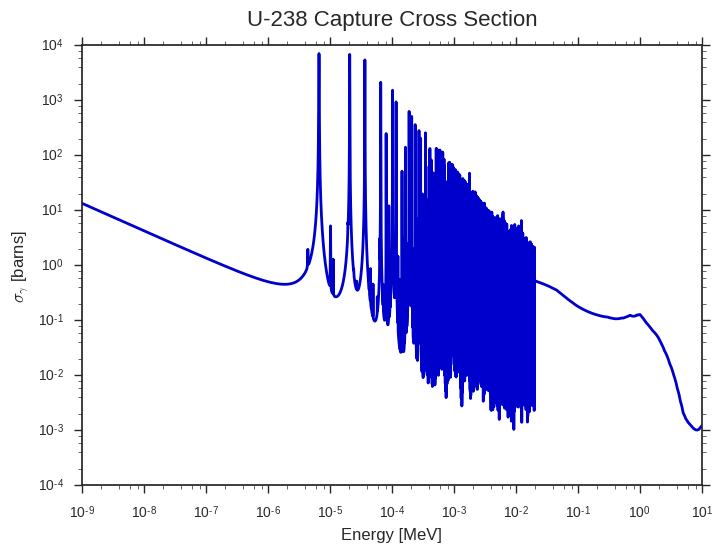
\includegraphics[width=0.8\linewidth]{figures/mgxs/u238-capture-xs}
\caption[U-238 capture cross section]{The continuous energy capture cross section for U-238.}
\label{fig:chap2-u238-xs}
\end{figure}
 
Although cross sections are experimentally measured, the neutron flux must be calculated analytically or with simulation. The steady-state continuous energy transport equation is integro-differential in the neutron angular flux $\psi(\mathbf{r},\mathbf{\Omega},E)$ and balances the rate of change of the population of neutrons in phase space to the difference between the production and loss rates of neutrons within a closed system:

\begin{dmath}
\label{eqn:chap1-transport-ce}
\mathbf{\Omega} \cdot \nabla \psi(\mathbf{r},\mathbf{\Omega},E) + \Sigma_{t}(\mathbf{r},E)\psi(\mathbf{r},\mathbf{\Omega},E) \;\;\;\;\; = \;\;\;\;\; \int\displaylimits_{0}^{\infty}\int\displaylimits_{4\pi} \Sigma_{s}(\mathbf{r},{\mathbf{\Omega'}\rightarrow\mathbf{\Omega}},{E'\rightarrow E}) \psi(\mathbf{r},\mathbf{\Omega'},E') \mathrm{d}\mathbf{\Omega'} \mathrm{d}E' + Q(\mathbf{r},\mathbf{\Omega},E)
\end{dmath}

The first term on the left hand side of the equation represents the streaming of neutrons within space and the second term is the total neutron collision rate determined by the total cross section $\Sigma_{t}$. On the right hand side, the first term models the scattering of neutrons at energy $E'$ and direction $\mathbf{\Omega'}$ into some new energy $E$ and direction $\mathbf{\Omega}$. The final term represents a generic source $Q$ of neutrons. In the case of critical systems, such as nuclear reactors, $Q$ is a source of fission neutrons:

\begin{dmath}
\label{eqn:chap1-source}
Q(\mathbf{r},\mathbf{\Omega},E) = \frac{1}{k_{eff}}\int\displaylimits_{0}^{\infty}\int\displaylimits_{4\pi} \nu\Sigma_{f}(\mathbf{r},{\Omega'\rightarrow \Omega},{E'\rightarrow E})\psi(\mathbf{r},\mathbf{\Omega'},E') \mathrm{d}\mathbf{\Omega'} \mathrm{d}E'
\end{dmath}

The $\nu\Sigma_{f}$ cross section is the probability of neutrons of energy $E$ and angle $\Omega$ resulting from fission at $E'$ and $\Omega'$. The eigenvalue $k_{eff}$ of a critical system represents the multiplication of neutrons from fission and balances neutron sources with losses due to absorption and leakage.

A solution for the neutron flux must computed from the transport equation. The accurate determination of the reaction rate distribution is primarily challenged by  the complicated energy structure of the cross sections. In addition, the distribution of neutrons in \ac{LWRs} spans 11 orders of magnitude from a few MeV at birth from fission emission to death by absorption at energies which approach 0 eV. As a result, analytical solutions to Eqn.~\ref{eqn:chap1-transport-ce} are intractable without significant simplifying assumptions.

Instead, numerical simulation is used to solve the transport equation for the flux. Monte Carlo techniques may be employed to exactly treat the energy dependence in Eqn.~\ref{eqn:chap1-transport-ce}\footnote{The treatment is only as exact as the uncertainties in measured nuclear cross section data will permit.}, but are computationally burdensome and impractical for routine nuclear reactor analysis. Although space and angle may be discretized using standard techniques for the solution of PDEs, special treatment must be given to the angular and energy variables as discussed in the following sections.


%%%%%%%%%%%%%%%%%%%%%%%%%%%%%%%%%%%%%%%%%%%%%%%%%%%%%%%%%%%%%%%%%%%%%%%%%%%%%%%
\section{Approximations in Angle}
\label{sec:chap2-angle}

%%%%%%%%%%%%%%%%%%%%%%%%%%%
\subsection{Isotropic Fission Source}
\label{subsec:chap2-fiss-src}

The neutrons emitted from fission form a nearly isotropic distribution independent of the energy or angle of the incoming neutron. As a result, the fission production cross section can be approximated as $\nu\Sigma_{f}(\mathbf{r},{\Omega'\rightarrow \Omega},{E'\rightarrow E}) \approx \nu\Sigma_{f}(\mathbf{r},{E'\rightarrow E})$. This permits the fission source in Eqn.~\ref{eqn:chap1-source} to be written as:

\begin{dmath}
\label{eqn:chap1-source-scalar-flux}
Q(\mathbf{r},\mathbf{\Omega},E) = \frac{1}{4\pi k_{eff}}\int\displaylimits_{0}^{\infty}\int\displaylimits_{4\pi} \nu\Sigma_{f}(\mathbf{r},{E'\rightarrow E})\psi(\mathbf{r},\mathbf{\Omega'},E') \mathrm{d}\mathbf{\Omega'} \mathrm{d}E'
\end{dmath}

The isotropic approximation reduces the dimensionality of the fission production cross section and simplifies the derivation of the approximations in the following sections.

% such that $\nu\Sigma_{f}(\mathbf{r},{\Omega'\rightarrow \Omega},{E'\rightarrow E}) \approx \nu\Sigma_{f}(\mathbf{r},{E'\rightarrow E})$. 

% in terms of the scalar flux $\phi(\mathbf{r},E)$:

%\begin{dmath}
%\label{eqn:chap1-source-scalar-flux}
%Q(\mathbf{r},\mathbf{\Omega},E) = \frac{1}{4\pi k_{eff}} \int\displaylimits_{0}^{\infty}\nu\Sigma_{f}(\mathbf{r},{E'\rightarrow E})\phi(\mathbf{r},E') \mathrm{d}E'
%\end{dmath}

%\begin{dmath}
%\label{eqn:chap1-scalar-flux}
%\phi_{g}(\mathbf{r},E) = \int\displaylimits_{4\pi}\psi(\mathbf{r},\Omega,E)\mathrm{d}\Omega
%\end{dmath}


%%%%%%%%%%%%%%%%%%%%%%%%%%%%%%
\subsection{Scattering Source}
\label{subsec:chap2-scatt-src}

-expand angular flux using spherical harmonics as basis functions of the angular dependence\\
-perhaps leave angular dependence in general form of transport equation above\\
-then use two subsections to describe the angular expansion of the scattering source, and the isotropy of the fission source?\\


%%%%%%%%%%%%%%%%%%%%%%%%%%%%%%%%%%%%%%%%%%%%%%%%%%%%%%%%%%%%%%%%%%%%%%%%%%%%%%%
\section{Multi-Group Theory}
\label{sec:chap2-mg-theory}

%%%%%%%%%%%%%%%%%%%%%%%%%%%%%%%%%%
\subsection{Energy Discretization}
\label{sec:chap2-energy}

The multi-group approach used to solve the transport equation subdivides the neutron's energy into discrete bins known as energy groups. The energy groups are indexed starting at 1 for high energies and ending with $G$ for the lowest energies of interest. An energy group $g \in \left\{1, 2, \ldots, G\right\}$  spans a range of energies from $\left[E_{g}, E_{g-1}\right]$ where $E_{0}$ is the lowest energy under consideration\footnote{Although $E_{0}$ is often taken to be zero, this may not be appropriate in practice since cross sections can only be accurately measured for finite neutron energies.} and $E_{g}$ is the upper bound of group $g$. First, a group-wise angular flux $\psi_{g}$ is defined for each energy group:

\begin{dmath}
\label{eqn:chap1-groupwise-flux}
\psi_{g}(\mathbf{r},\mathbf{\Omega}) = \int\displaylimits_{E_{g}}^{E_{g-1}} \psi(\mathbf{r},\mathbf{\Omega},E)\mathrm{d}E
\end{dmath}

%A group-wise scalar flux $\phi_{g}$ can be similarly defined.

Next, the continuous energy transport equation (Eqn.~\ref{eqn:chap1-transport-ce}) with a fission source (Eqn.~\ref{eqn:chap1-source}) can be transformed into its multi-group form by first integrating over each energy group:

\begin{dmath}
\label{eqn:chap1-transport-mg-1}
\mathbf{\Omega} \cdot \nabla \psi_{g}(\mathbf{r},\mathbf{\Omega}) + \int\displaylimits_{E_{g}}^{E_{g-1}} \Bigg[\Sigma_{t}(\mathbf{r},E)\psi(\mathbf{r},\mathbf{\Omega},E)\Bigg]\mathrm{d}E = \;\;\; \int\displaylimits_{E_{g}}^{E_{g-1}} \Bigg[\sum_{g'=1}^{G} \int\displaylimits_{E_{g'}}^{E_{g'-1}}\int\displaylimits_{4\pi} \Sigma_{s}(\mathbf{r},{\mathbf{\Omega'}\rightarrow\mathbf{\Omega}},{E'\rightarrow E}) \psi(\mathbf{r},\mathbf{\Omega'},E') \mathrm{d}\mathbf{\Omega'} \mathrm{d}E'\Bigg]\mathrm{d}E + 
\int\displaylimits_{E_{g}}^{E_{g-1}}\Bigg[\frac{1}{4\pi k_{eff}}\sum_{g'=1}^{G} \int\displaylimits_{E_{g'}}^{E_{g'-1}}\int\displaylimits_{4\pi}\nu\Sigma_{f}(\mathbf{r},{E'\rightarrow E})\psi(\mathbf{r},\mathbf{\Omega'},E')\mathrm{d}\mathbf{\Omega'}\mathrm{d}E'\Bigg]\mathrm{d}E
\end{dmath}

The integrals in Eqn.~\ref{eqn:chap1-transport-mg-1} over incoming neutron energy in the scattering kernel and fission source are treated as summations of discrete integrals over each incoming energy group. Although the streaming term is easily expressed in terms of the multi-group flux $\psi_{g}$, the total collision, scattering and fission terms are defined as integral quantities. These three terms can be simplified by multiplying each by unity in the form of $\nicefrac{\psi_{g}}{\psi_{g}}$:

\begin{dmath}
\label{eqn:chap1-transport-mg-2}
\mathbf{\Omega} \cdot \nabla \psi_{g}(\mathbf{r},\mathbf{\Omega}) + \ddfrac{\int\displaylimits_{E_{g}}^{E_{g-1}} \Sigma_{t}(\mathbf{r},E)\psi(\mathbf{r},\mathbf{\Omega},E)\mathrm{d}E}{\psi_{g}(\mathbf{r},\mathbf{\Omega})}\psi_{g}(\mathbf{r},\mathbf{\Omega}) 
= \;\;\; 
\sum_{g'=1}^{G} \ddfrac{\int\displaylimits_{E_{g}}^{E_{g-1}} \int\displaylimits_{E_{g'}}^{E_{g'-1}}\int\displaylimits_{4\pi} \Sigma_{s}(\mathbf{r},{\mathbf{\Omega'}\rightarrow\mathbf{\Omega}},{E'\rightarrow E}) \psi(\mathbf{r},\mathbf{\Omega'},E') \mathrm{d}\mathbf{\Omega'} \mathrm{d}E'}{\psi_{g'}(\mathbf{r},\mathbf{\Omega'})}\psi_{g'}(\mathbf{r},\mathbf{\Omega'})
+ 
\dfrac{1}{4\pi k_{eff}} \sum_{g'=1}^{G} \ddfrac{\int\displaylimits_{E_{g}}^{E_{g-1}} \int\displaylimits_{E_{g'}}^{E_{g'-1}}\int\displaylimits_{4\pi} \nu\Sigma_{f}(\mathbf{r},{E'\rightarrow E})\psi(\mathbf{r},\mathbf{\Omega'},E') \mathrm{d}\mathbf{\Omega'} \mathrm{d}E'\mathrm{d}E}{\psi_{g'}(\mathbf{r},\mathbf{\Omega'})}\psi_{g'}(\mathbf{r},\mathbf{\Omega'})
\end{dmath}

The fractional terms in the Eqn.~\ref{eqn:chap1-transport-mg-2} are defined as the \ac{MGXS} for total, scattering and fission production reactions. The \ac{MGXS} are the averages of the corresponding continuous energy cross sections weighted by the angular neutron flux $\psi$ in each energy group. The \ac{MGXS} $\Sigma_{t,g}$, $\Sigma_{s,g' \rightarrow g}$ and $\nu\Sigma_{f,g' \rightarrow g}$ are defined below for completeness:

\begin{dmath}
\label{eqn:chap1-sigt-mg}
\Sigma_{t,g}(\mathbf{r},\mathbf{\Omega}) \equiv \frac{\int\displaylimits_{E_{g}}^{E_{g-1}} \Sigma_{t}(\mathbf{r},E)\psi(\mathbf{r},\mathbf{\Omega},E)\mathrm{d}E}{\psi_{g}(\mathbf{r},\mathbf{\Omega})}
\end{dmath}

\begin{dmath}
\label{eqn:chap1-sigs-mg}
\Sigma_{s,g' \rightarrow g}(\mathbf{r},\mathbf{\Omega}) \equiv \frac{\int\displaylimits_{E_{g}}^{E_{g-1}} \int\displaylimits_{E_{g'}}^{E_{g'-1}}\int\displaylimits_{4\pi} \Sigma_{s}(\mathbf{r},{\mathbf{\Omega'}\rightarrow\mathbf{\Omega}},{E'\rightarrow E}) \psi(\mathbf{r},\mathbf{\Omega'},E') \mathrm{d}\mathbf{\Omega'} \mathrm{d}E' \mathrm{d}E} {\psi_{g'}(\mathbf{r},\mathbf{\Omega'})}
\end{dmath}

\begin{dmath}
\label{eqn:chap1-nusigf-mg}
\nu\Sigma_{f,g' \rightarrow g}(\mathbf{r},\mathbf{\Omega}) \equiv \frac{\int\displaylimits_{E_{g}}^{E_{g-1}} \int\displaylimits_{E_{g'}}^{E_{g'-1}}\int\displaylimits_{4\pi} \nu\Sigma_{f}(\mathbf{r},{E'\rightarrow E})\psi(\mathbf{r},\mathbf{\Omega'},E') \mathrm{d}\mathbf{\Omega'} \mathrm{d}E'\mathrm{d}E}{\psi_{g'}(\mathbf{r},\mathbf{\Omega'})}
\end{dmath}

With these definitions of the \ac{MGXS}, the multi-group form of the transport equation in Eqn.~\ref{eqn:chap1-transport-mg-1} can be expressed succinctly in terms of the group-wise angular flux $\psi_{g}$:

\begin{dmath}
\label{eqn:chap1-transport-mg-3}
\mathbf{\Omega} \cdot \nabla \psi_{g}(\mathbf{r},\mathbf{\Omega}) + \Sigma_{t,g}(\mathbf{r},E)\psi_{g}(\mathbf{r},\mathbf{\Omega}) =
\sum_{g'=1}^{G} \int\displaylimits_{4\pi} \Sigma_{s,g' \rightarrow g}(\mathbf{r},{\mathbf{\Omega'}\rightarrow\mathbf{\Omega}}) \psi_{g}(\mathbf{r},\mathbf{\Omega'}) \mathrm{d}\mathbf{\Omega'} + \frac{1}{4\pi k_{eff}}\sum_{g'=1}^{G} \int\displaylimits_{4\pi} \nu\Sigma_{f,g' \rightarrow g}(\mathbf{r})\psi_{g}(\mathbf{r},\mathbf{\Omega'}) \mathrm{d}\mathbf{\Omega'}
\end{dmath}

Thus far, no approximations have been made in the energy discretization of multi-group transport equation given in Eqn.~\ref{eqn:chap1-transport-mg-3}. However, the expressions for the \ac{MGXS} $\Sigma_{t,g}$, $\Sigma_{s,g' \rightarrow g}$ and $\nu\Sigma_{f,g' \rightarrow g}$ in Eqns.~\Crefrange{eqn:chap1-sigt-mg}{eqn:chap1-nusigf-mg} present a complication since they are dependent on the unknown angular flux as discussed in the following section.

-should I expand in angular moments first?\\
-it's not appropriate to simply remove the energy dependence in the scattering cross section is it?\\


%%%%%%%%%%%%%%%%%%%%%%%%%%%%%%
\subsection{Flux Separability Approximation}
\label{sec:chap2-angle}

The angular dependence of the \ac{MGXS} is commonly treated with the flux separability approximation. Flux separability makes the simplifying assumption that the energy and angular dependence of the flux varies independently such that the angular flux can be written as the product of the scalar neutron flux $\phi(\mathbf{r},E)$ and some function $W(\mathbf{r}, \mathbf{\Omega})$:

\begin{dmath}
  \label{eqn:chap1-flux-separate}
  \psi(\mathbf{r},\mathbf{\Omega},E) = \phi(\mathbf{r},E) W(\mathbf{r},\mathbf{\Omega})
\end{dmath}

\begin{dmath}
\label{eqn:chap1-scalar-flux}
\phi(\mathbf{r},E) = \int\displaylimits_{4\pi} \psi(\mathbf{r},\mathbf{\Omega},E)\mathrm{d}\mathbf{\Omega}
\end{dmath}

The angular dependence of the \ac{MGXS} is eliminated by inserting Eqn.~\ref{eqn:chap1-flux-separate} into Eqns.~\cref{eqn:chap1-sigt-mg,eqn:chap1-sigs-mg,eqn:chap1-nusigf-mg}, factoring out $W(\mathbf{r}, \mathbf{\Omega})$ and writing the \ac{MGXS} in terms of the scalar flux:

% $\phi(\mathbf{r},E)$:

\begin{dmath}
\label{eqn:chap1-sigt-mg-scalar}
\Sigma_{t,g}(\mathbf{r}) \equiv \frac{\int\displaylimits_{E_{g}}^{E_{g-1}} \Sigma_{t}(\mathbf{r},E)\phi(\mathbf{r},E)\mathrm{d}E}{\phi_{g}(\mathbf{r})}
\end{dmath}

\begin{dmath}
\label{eqn:chap1-sigs-mg-scalar}
\Sigma_{s,g' \rightarrow g}(\mathbf{r}) \equiv \frac{\int\displaylimits_{E_{g}}^{E_{g-1}} \int\displaylimits_{E_{g'}}^{E_{g'-1}} \Sigma_{s}(\mathbf{r},{E'\rightarrow E}) \phi(\mathbf{r},E') \mathrm{d}E' \mathrm{d}E} {\phi_{g'}(\mathbf{r})}
\end{dmath}

\begin{dmath}
\label{eqn:chap1-nusigf-mg-scalar}
\nu\Sigma_{f,g' \rightarrow g}(\mathbf{r}) \equiv \frac{\int\displaylimits_{E_{g}}^{E_{g-1}} \int\displaylimits_{E_{g'}}^{E_{g'-1}} \nu\Sigma_{f}(\mathbf{r},{E'\rightarrow E})\phi(\mathbf{r},E') \mathrm{d}E'\mathrm{d}E}{\phi_{g'}(\mathbf{r})}
\end{dmath}

%The group-wise scalar flux $\phi_{g}$ is the corollary to its angle dependent counterpart $\psi_{g}$:

%\begin{dmath}
%\label{eqn:chap1-scalar-flux-mg}
%\phi_{g}(\mathbf{r}) = \int\displaylimits_{E_{g}}^{E_{g-1}}\phi(\mathbf{r},E)\mathrm{d}E
%\end{dmath}

-mention that this approx. will be reivisited in later sections\\
-refer to consistent-p approximation \\
-cite nuclear eng handbook?\\



%%%%%%%%%%%%%%%%%%%%%%%%%%%%%%%%%%%
\subsection{Spatial Homogenization}
\label{sec:chap2-space}

%Up to this point the \ac{MGXS} have been defined as continuously varying in space. Most deterministic methods solve the multi-group transport equation by discretizing the spatial domain. The following equation introduces an integral over each mesh cell $i$ to each term in the multi-group transport equation:

%\begin{dmath}
%\label{eqn:chap1-transport-mg-4}
%\int\displaylimits_{\mathbf{r} \in V_{i}}\left(\mathbf{\Omega} \cdot \nabla \psi_{g}(\mathbf{r},\mathbf{\Omega}) + \Sigma_{t,g}(\mathbf{r})\psi_{g}(\mathbf{r},\mathbf{\Omega})\right)\mathrm{d}\mathbf{r} \;\;\;\; = \;\;\;\;\; \int\displaylimits_{\mathbf{r} \in V_{i}}\sum_{g'=1}^{G} \int\displaylimits_{4\pi} \Sigma_{s,g' \rightarrow g}(\mathbf{r},{\mathbf{\Omega'}\rightarrow\mathbf{\Omega}}) \psi_{g}(\mathbf{r},\mathbf{\Omega'}) \mathrm{d}\mathbf{\Omega'} \mathrm{d}\mathbf{r} + \frac{1}{4\pi k_{eff}}\int\displaylimits_{\mathbf{r} \in V_{i}}\sum_{g'=1}^{G} \int\displaylimits_{4\pi} \nu\Sigma_{f,g' \rightarrow g}(\mathbf{r})\psi_{g}(\mathbf{r},\mathbf{\Omega'}) \mathrm{d}\mathbf{\Omega'} \mathrm{d}\mathbf{r}
%\end{dmath}

Up to this point the \ac{MGXS} have been defined as continuously varying in space. In practice, most deterministic methods used to solve the multi-group transport equation make the simplifying assumption that the material properties are constant across each mesh cell. Spatial homogenization is used to to compute flux-weighted volume-averaged cross sections within each mesh cell $i$ with volume $V_{i}$ as follows:

\begin{dmath}
\label{eqn:chap1-sigt-mg-scalar}
\Sigma_{t,i,g} = \frac{\int\displaylimits_{\mathbf{r} \in V_{i}}\int\displaylimits_{E_{g}}^{E_{g-1}} \Sigma_{t}(\mathbf{r},E)\phi(\mathbf{r},E)\mathrm{d}E\mathrm{d}\mathbf{r}}{\int\displaylimits_{\mathbf{r} \in V_{i}}\phi_{g}(\mathbf{r})\mathrm{d}\mathbf{r}}
\end{dmath}

\begin{dmath}
\label{eqn:chap1-sigs-mg-scalar}
\Sigma_{s,i,g' \rightarrow g} \equiv \frac{\int\displaylimits_{\mathbf{r} \in V_{i}}\int\displaylimits_{E_{g}}^{E_{g-1}} \int\displaylimits_{E_{g'}}^{E_{g'-1}} \Sigma_{s}(\mathbf{r},{E'\rightarrow E}) \phi(\mathbf{r},E') \mathrm{d}E' \mathrm{d}E\mathrm{d}\mathbf{r}}{\int\displaylimits_{\mathbf{r} \in V_{i}}\phi_{g'}(\mathbf{r})\mathrm{d}\mathbf{r}}
\end{dmath}

\begin{dmath}
\label{eqn:chap1-nusigf-mg-scalar}
\nu\Sigma_{f,i,g' \rightarrow g} \equiv \frac{\int\displaylimits_{\mathbf{r} \in V_{i}}\int\displaylimits_{E_{g}}^{E_{g-1}} \int\displaylimits_{E_{g'}}^{E_{g'-1}} \nu\Sigma_{f}(\mathbf{r},{E'\rightarrow E})\phi(\mathbf{r},E') \mathrm{d}E'\mathrm{d}E\mathrm{d}\mathbf{r}}{\int\displaylimits_{\mathbf{r} \in V_{i}}\phi_{g'}(\mathbf{r})\mathrm{d}\mathbf{r}}
\end{dmath}

A variety of discretization schemes may be used to solve the following multi-group transport equation in Eqn.~\ref{eqn:chap1-transport-mg-3}, including the \ac{MOC} and discrete ordinates (S$_N$). For first order discretization schemes in space, the transport equation can be re-written in terms of the volume-averaged group-wise fluxes $\psi_{i,g}$ and the spatially homogenized \ac{MGXS} in each mesh cell and energy group:

\begin{dmath}
\label{eqn:chap1-transport-mg-4}
\mathbf{\Omega} \cdot \nabla \psi_{i,g}(\mathbf{\Omega}) + \Sigma_{t,i,g}\psi_{i,g}(\mathbf{\Omega}) \;\;\;\; = \;\;\;\;\;
\sum_{g'=1}^{G} \int\displaylimits_{4\pi} \Sigma_{s,i,g' \rightarrow g}({\mathbf{\Omega'}\rightarrow\mathbf{\Omega}}) \psi_{i,g}(\mathbf{\Omega'}) \mathrm{d}\mathbf{\Omega'} + 
\frac{1}{4\pi k_{eff}}\sum_{g'=1}^{G} \int\displaylimits_{4\pi} \nu\Sigma_{f,i,g' \rightarrow g}\psi_{i,g}(\mathbf{\Omega'}) \mathrm{d}\mathbf{\Omega'}
\end{dmath}

This is the form of the multi-group transport equation solved using the deterministic OpenMOC code in this thesis. 


\begin{itemize}[noitemsep]
  \item use $x$ in place of $t$ for general \ac{MGXS}?
  \item equation and figures mapped to variables
  \item tally ``noise'' model
  \item uncertainty propagation equations
  \item mention that this intro is agnostic to the method used to solve the transport eqn.
   \item in constant-in-angle section, mention Nate Eqn. 1.13 as one possible approach for deterministic methods for the collapse. In MC we use the angular flux in the collapse though.
   \item cite boltzmann transport equation (see adam's thesis pg. 1) 
   \item mention recent work to use MC for MGXS (chap. 3 of nelson's thesis)
   \item define angular flux - neutron angular density multiplied by neutron speed
   \item phase space defn from adam's thesis pg 5 - as tot dist traveled
   \item talk about (n,xn) reactions
   \item keep fission as matrix early on
   \item figure 2.2 from adam's thesis to describe typical approach
\end{itemize}


%%%%%%%%%%%%%%%%%%%%%%%%%%%%%%%%%%%
\subsection{Scattering Production}
\label{sec:chap2-scatt-prod}

Although neutron production is dominated by fission in nuclear reactors, there may also be non-negligible production of neutrons due to scattering multiplicity $(n,xn)$ reactions. Production from scattering is typically accounted for with a factor $\nu_{scatt,i,g' \rightarrow g}$ which represents the average number of neutrons produced in a scattering reaction. The factor $\nu_{scatt,i,g' \rightarrow g}$ may be lumped into the scattering matrix $\nu_{scatt,i,g' \rightarrow g}\Sigma_{s,i,g' \rightarrow g}$ and substituted directly into the scattering source term in the multi-group transport equation. 

The $k_{eff}$ eigenvalue is only defined for fission operator in the transport equation. As a result, deterministic methods which compute the eigenvalue using the fission production, absorption and leakage rates will fail to capture the scattering production in in the multiplication factor. In order to account for $(n,xn)$ reactions, a ``corrected'' absorption cross section $\tilde{\Sigma}_{a,i,g} = \Sigma_{a,i,g} - (1-\nu_{scatt,i,g' \rightarrow g})\Sigma_{s,i,g' \rightarrow g}$ must be used to preserve neutron balance. Alternatively, $(n,xn)$ reactions will be accounted for if the eigenvalue is computed as the ratio of successive fission sources in iterative deterministic methods.


%%%%%%%%%%%%%%%%%%%%%%%%%%%%%%%%%%%
\subsection{Fission Matrix Condensation}
\label{sec:chap2-fiss-mat}

The scattering and fission production matrices dominate the memory storage requirements for \ac{MGXS} since they depend on both incoming and outgoing energy groups. In thermal reactors the energy distribution of neutrons produced in fission is nearly independent of the incoming neutron energy, and the fission production matrix can be condensed into two single dimensional vectors for each energy group. The fission spectrum $\chi_{g}$ is introduced as a probability distribution over outgoing fission energies:

\begin{dmath}
\label{eqn:chap1-nusifg}
\chi_{g} \equiv \frac{\displaystyle\sum\limits_{g'=1}^{G}\nu\Sigma_{f,g'\rightarrow g}\phi_{g'}}{\displaystyle\sum\limits_{g=1}^{G}\displaystyle\sum\limits_{g'=1}^{G}\nu\Sigma_{f,g'\rightarrow g}}
\end{dmath}

The group-wise fission production cross section $\nu\Sigma_{f,g}$ is defined as the flux-weighted sum of $\nu\Sigma_{f,g'\rightarrow g}$ over all outgoing groups:

% and signifies the probability of fission occurring in group $g$:

\begin{dmath}
\label{eqn:chap1-nusifg}
\nu\Sigma_{f,g'} \equiv \displaystyle\sum\limits_{g'=1}^{G}\nu\Sigma_{f,g'\rightarrow g}\phi_{g'}
\end{dmath}

Upon substituting $\chi_{g}$ and $\nu\Sigma_{f,g}$ into Eqn.~\ref{eqn:chap1-transport-mg-4} one obtains:

\begin{dmath}
\label{eqn:chap1-transport-mg-6}
\mathbf{\Omega} \cdot \nabla \psi_{g}(\mathbf{r},\mathbf{\Omega}) + \Sigma_{t,i,g}\psi_{g}(\mathbf{r},\mathbf{\Omega}) \;\;\;\; = \;\;\;\;\;
\sum_{g'=1}^{G} \int\displaylimits_{4\pi} \Sigma_{s,i,g' \rightarrow g}(\mathbf{r},{\mathbf{\Omega'}\rightarrow\mathbf{\Omega}}) \psi_{g}(\mathbf{r},\mathbf{\Omega'}) \mathrm{d}\mathbf{\Omega'} + 
\frac{\chi_{i,g}}{4\pi k_{eff}}\sum_{g'=1}^{G} \int\displaylimits_{4\pi} \nu\Sigma_{f,i,g}\psi_{g}(\mathbf{r},\mathbf{\Omega'}) \mathrm{d}\mathbf{\Omega'}
\end{dmath}


%frequently made in multi-group transport calculations thermal reactor spectra the energy distribution of neutrons produced in fission is nearly independent of the incoming neutron energy.

%to reduce the dimensionality of the fission production matrix $\nu\Sigma_{f,g'\rightarrow g}$. In thermal reactor spectra the energy distribution of neutrons produced in fission is nearly independent of the incoming neutron energy.


%%%%%%%%%%%%%%%%%%%%%%%%%%%
\subsection{Approximations}
\label{subsec:chap2-approx}

Although \autoref{eqn:moc-theory-condensed-chi} assumes a dependence of $\chi$ on both the energy of the neutron causing fission $g'$ and the fission emission energy group $g$, the former is typically summed over to simplify the multi-group $\chi$ to the following approximation:

\begin{equation}
\label{eqn:moc-theory-condensed-chi-group}
\chi_{g}(\mathbf{r}) = \displaystyle\sum\limits_{g=1}^{G}\chi_{g'\rightarrow g}(\mathbf{r})
\end{equation}


%%%%%%%%%%%%%%%%%%%%%%%%%%%%%%%%%%%%
\subsubsection{Isotropic Scattering}
\label{subsubsec:chap2-iso-scatter}

\begin{itemize}
  \item mention ``iso-in-lab'' feature in OpenMC
\end{itemize}


%%%%%%%%%%%%%%%%%%%%%%%%%%%%%%%%%%%%%%%%%%%%%%%%%%%%%%%%%%%%%%%%%%%%%%%%%%%%%%%
\section{MGXS Generation with Monte Carlo}
\label{sec:chap2-mgxs-mc}

\begin{itemize}[noitemsep]
  \item \ac{MC} is \emph{reactor agnostic}
  \item stochastic approx. to integrals in Section~\ref{sec:chap2-background}
\end{itemize}

%%%%%%%%%%%%%%%%%%%%%%
\subsection{Past Work}
\label{subsec:chap2-past-work}

\begin{itemize}[noitemsep]
  \item \ac{MGXS} for coarse mesh diffusion
  \begin{itemize}[noitemsep]
    \item Redmond
    \item Pounders
    \item Serpent
  \end{itemize}
  \item \ac{MGXS} for fine mesh transport
  \begin{itemize}[noitemsep]
    \item Nelson with NDPP
  \end{itemize}
\end{itemize}

%%%%%%%%%%%%%%%%%%%%%%%%%%%%%%%%%%%%%%%%%%%%%
\subsection{Spatial Self-Shielding Treatment}
\label{subsec:chap2-spatial-shield}

\begin{itemize}[noitemsep]
  \item spatial self-shielding treatment is natural in \ac{MC}
  \item challenge is slow convergence rate
  \item motivate clustering
\end{itemize}